\chapter{Исследовательская часть}

\section{Замеры времени работы}

Для замеров времени работы функции запускались 100 раз, на каждой итерации генерировались 2 строки одинаковой длины, состоящие из случайных цифр. Результаты измерений суммировались, после чего выводилось среднее значение. Время работы было замерено с помощью функции $ticks\_us()$ из модуля $utime$~\cite{utime}. Все замеры проводились на микропроцессоре $STM32F767ZIT6$.

При всех используемых вариантах замеры проводились на строках длины 1, 2, 3, 4, 5. Результаты представлены на рисунке~\ref{fig:res1}.

\begin{figure}[h!]
	\centering
	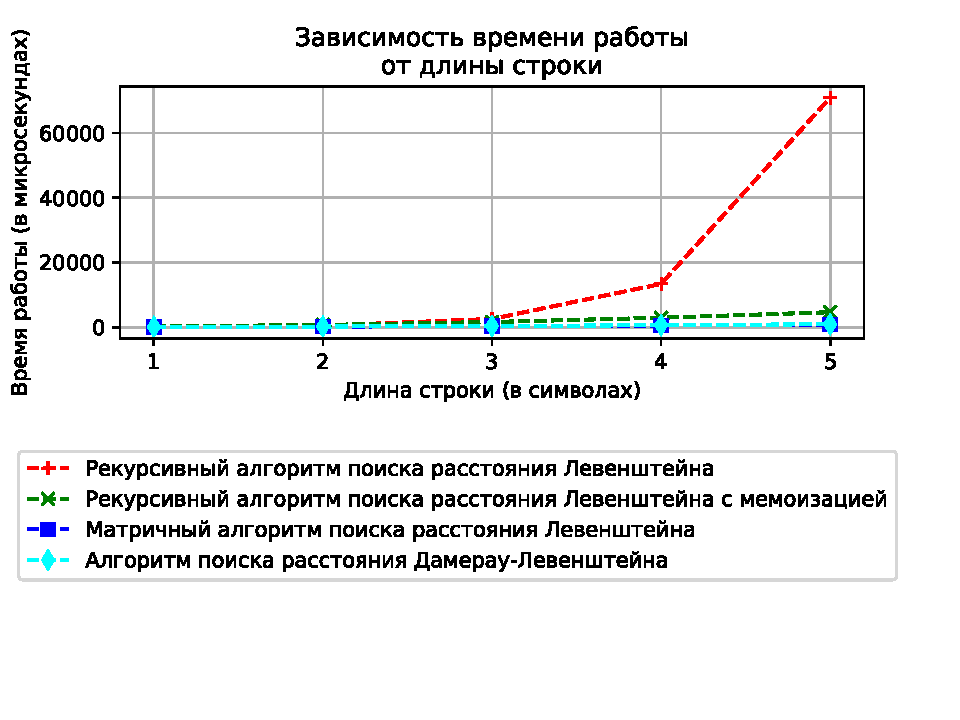
\includegraphics[width=0.9\textwidth]{tex_parts/research1.pdf}
	\caption{\label{fig:res1} Результаты замера времени работы разных алгоритмов на строках длины 1, 2, 3, 4, 5.}
\end{figure}

Рекурсивная реализация без мемоизации работает дольше остальных. Однако есть проблемы со сравнением других реализаций. На рисунке~\ref{fig:res2} представлены результаты для всех реализаций, кроме рекурсивной.

\begin{figure}[h!]
	\centering
	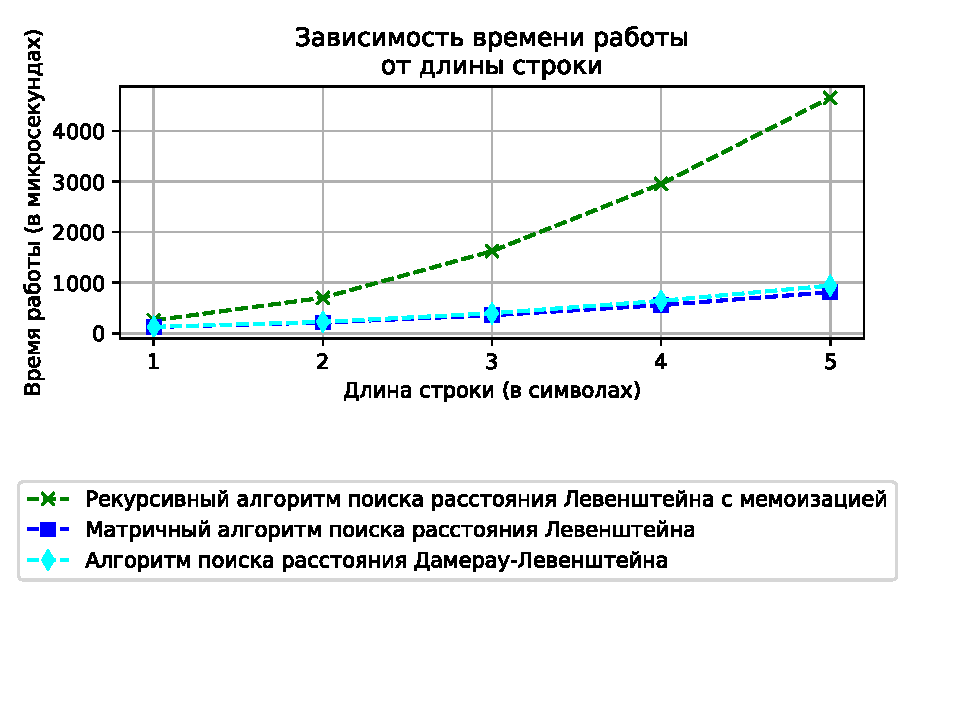
\includegraphics[width=0.9\textwidth]{tex_parts/research2.pdf}
	\caption{\label{fig:res2} Результаты замера времени работы разных алгоритмов на строках длины 1, 2, 3, 4, 5 (кроме рекурсивной реализации).}
\end{figure}

Наиболее эффективной по времени оказалась матричная реализация алгоритма поиска расстояния Левенштейна, наименее эффективной из оставшихся -- рекурсивный алгоритм с мемоизацией.

\section{Вывод}

В данном разделе были проведены замеры времени. Самыми эффективными оказались матричные реализации алгоритмов, причём расстояние Левенштейна считается быстрее, чем расстояние Дамерау-Левенштейна. Далее идёт рекурсивный алгоритм с мемоизацией, и самым медленной оказалась обычная рекурсивная реализация.

